
	Com o objetivo de obter conhecimento referente à solução prática proposta durante este trabalho, foi desenvolvida uma pequena prova de conceito durante a primeira etapa deste trabalho (TCC\_1). Nesta seção estão apresentadas as informações sobre o planejamento e condução da prova de conceito, assim como as informações importantes obtidas com a realização da mesma, caracterizadas como \textit{resultados da prova de conceito}.

	Esta seção está dividida entre \textit{planejamento e condução} da prova de conceito, \ref{sub:planejamento_e_condução}, e \textit{características técnicas} \ref{sub:características_técnicas}.

	\subsection{Planejamento e Condução} % (fold)
	\label{sub:planejamento_e_condução}

		Esta prova de conceito foi pensada com o objetivo de identificar algumas características básicas sobre a implementação de sistemas de navegação inteligente utilizando os kits de robótica Mindstorms, da Lego. Com este objetivo, a prova de conceito envolveu a análise de ferramentas utilizadas, como sensores e atuadores, o estudo e seleção da linguagem de programação a ser utilizada e alguns detalhes referentes à localização relativa de obstáculos.

		Para isso, buscou-se simular uma atividade básica na navegação e auto-localização na robótica. Atividade esta, que tem como objetivo identificar obstáculos ao redor do robô, levando em consideração a margem de erro, assim como todas as características presentes nos sensores e atuadores do kit. Ou seja, o robô é colocado em um ambiente desconhecido, onde o mesmo busca identificar obstáculos à sua volta, com o objetivo de definir uma saída, onde não se encontra nenhum obstáculo.

		O ambiente utilizado para a prova de conceito pode ser observado na Figura \ref{img:ambienteProva}. A montagem do robô utilizada nesta prova seguiu o estabelecido na seção \ref{sub:montagem_do_robô}, utilizando esteiras, um sonar para identificar a distância de obstáculos, um sensor de toque e sensores odométricos em cada motor.

		\begin{figure}[H]
			\centering
			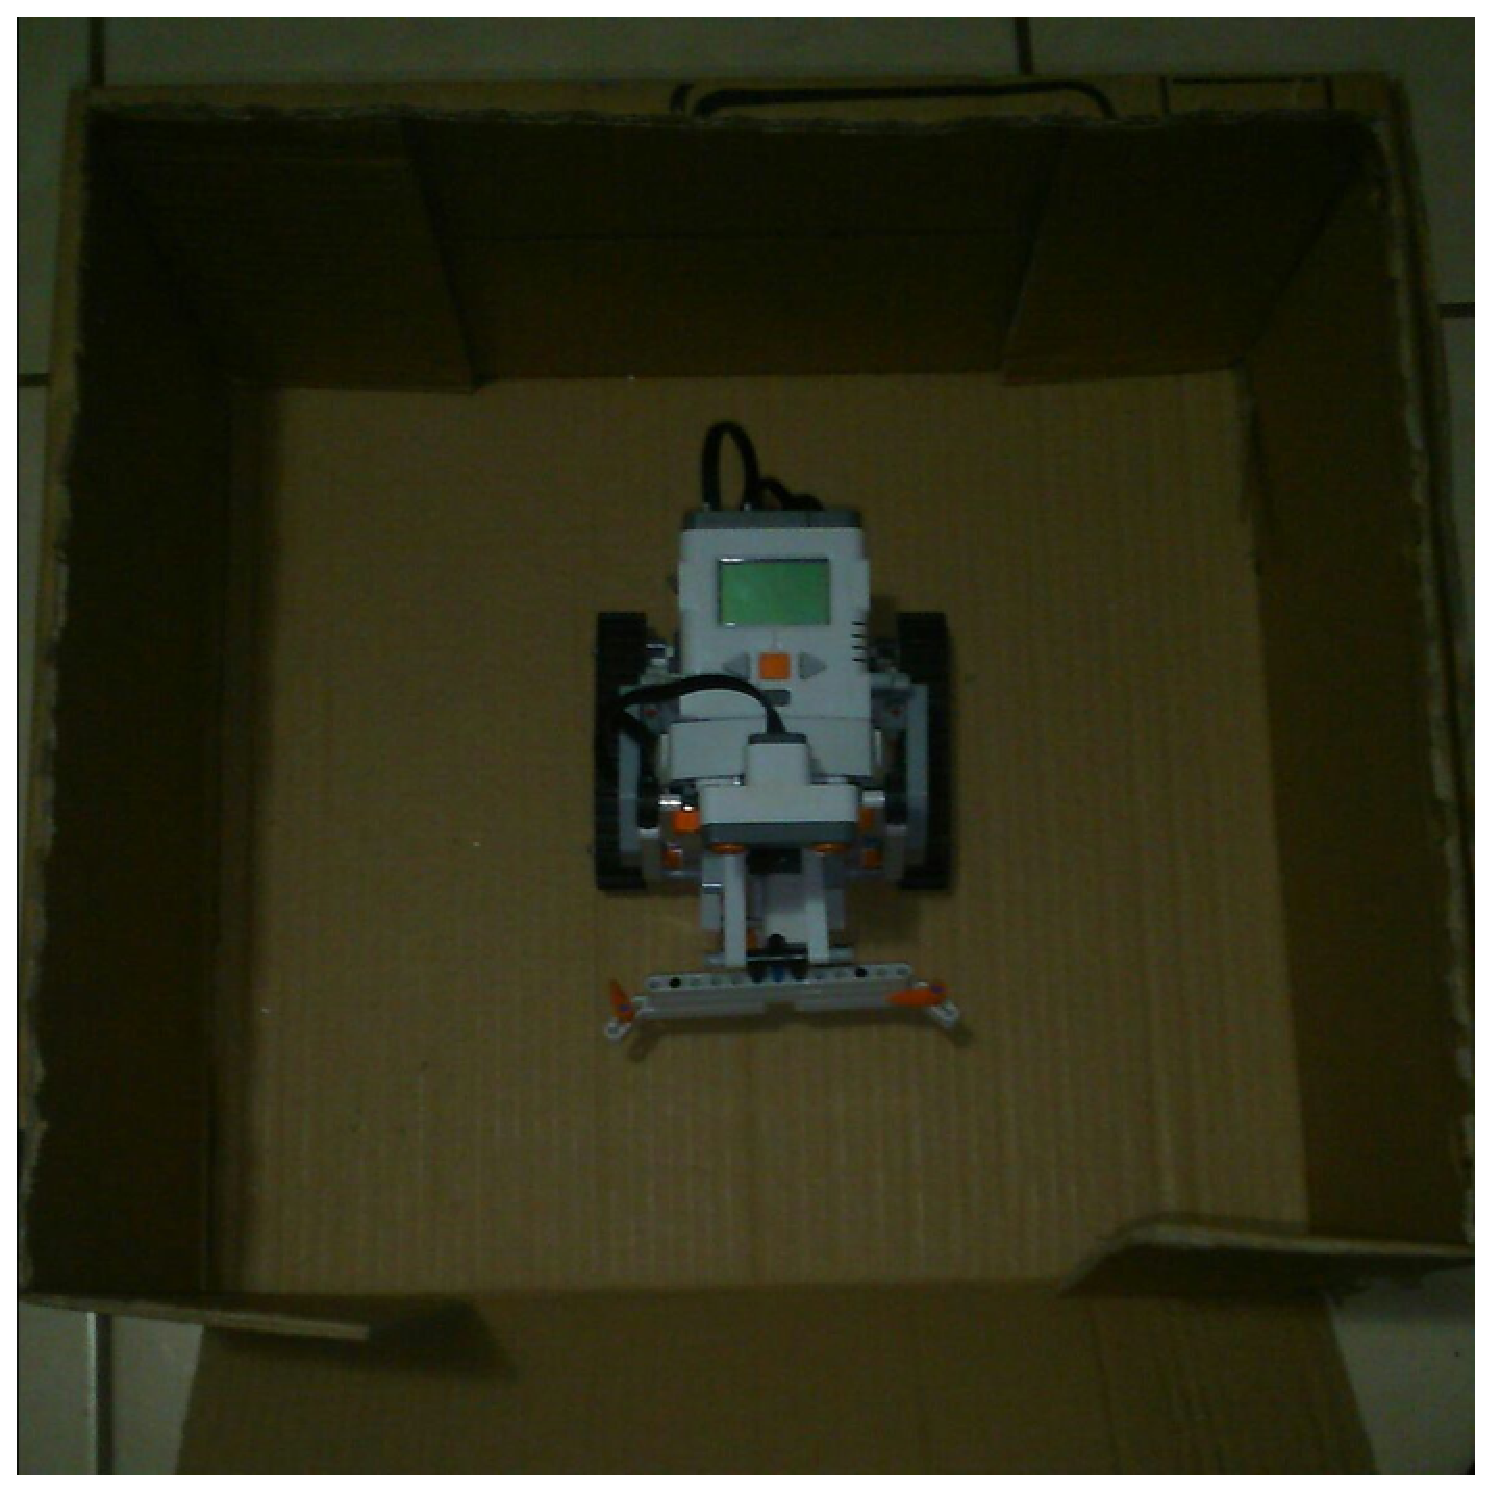
\includegraphics[scale=0.4]{figuras/ambienteConceito.eps}
			\label{img:ambienteProva}
			\caption{Ambiente Prova de Conceito}
		\end{figure}

		Com a realização da prova de conceito, ao implementar questões referentes ao posicionamento, direcionamento e localização do robô, diversas características foram identificadas e analisadas. Ao longo da seção \ref{sub:características_técnicas} estão apresentadas algumas destas características técnicas.

	% subsection planejamento_e_condução (end)

	\subsection{Características Técnicas} % (fold)
	\label{sub:características_técnicas}

		Neste tópico serão apresentadas algumas das características importantes identificadas durante a realização da prova de conceito.

		\subsubsection{Seleção da Linguagem e Ambiente de Desenvolvimento}

		Para realização desta prova de conceito, assim como o desenvolvimento de toda a solução proposta, ao longo do TCC\_2, optou-se pela utilização da linguagem Java. Esta escolha se deu não só devido à possibilidade, com mais facilidade, da integração desta solução com o \textit{framework} desenvolvido por \cite{tccRodrigo}, como também por todo o apoio técnico advindo da utilização da ferramenta \textit{leJOS NXJ}\footnote{http://www.lejos.org/nxj.php}.

		A ferramenta leJOS NXJ engloba, basicamente, uma máquina virtual Java (JVM) desenvolvida em C, sendo multiplataforma, ou seja, é portável para sistemas Linux, Windows e Macintosh \cite{legonxj}. O material de estudo sobre a ferramenta leJOS NXJ se encontra disponível em toda a \textit{web}, de maneira livre, e no livro \cite{legonxj}, que foi utilizado como fonte de informação durante o desenvolvimento.

		O sistema operacional utilizado para realização desta prova de conceito foi o \textit{windows}, devido a sua facilidade de configuração da comunicação entre robô/PC, diferentemente do observado em sistemas Linux. O \textit{passo-a-passo} para instalação e configuração do ambiente utilizado para desenvolvimento se encontra em \cite[p. 6]{legonxj}.

		A seleção desta ferramenta é decorrente, além dos motivos apresentados anteriormente, da existência de uma \textit{API} que disponibiliza diversas funcionalidades referentes à navegação dos robôs. A \textit{API} do leJOS NXJ engloba desde funções referentes ao controle de motores, até o apoio a criação de mapas e sistemas complexos de navegação.

		Em paralelo à escolha da linguagem de programação, buscou-se identificar um ambiente de desenvolvimento que disponibilizasse ferramentas de apoio que facilitem o desenvolvimento da solução. Com este objetivo, optou-se pela utilização da \textit{IDE} Eclipse\footnote{https://eclipse.org/}, por possuir um \textit{plugin} da ferramenta leJOS NXJ, como apresenta \cite{legonxj}. O tutorial para instalação e configuração do ambiente utilizado se encontra em \cite[p. 14]{legonxj}.

	\subsubsection{Atuadores}

		Os atuadores, ou motores, contemplam a base da robótica móvel. Desse modo, o leJOS NXT disponibiliza diversas funcionalidades referentes ao controle destes atuadores. Um exemplo disso é a possibilidade de controlar a aceleração do motor, possibilitando um arranque com aceleração gradual, para minimizar as chances de derrapagem, por exemplo.

		Estas possibilidades de controle de rotação são devido a existência de \textit{encoders} óticos em cada motor, como apresenta \cite{legonxj}. Cada \textit{encoder} tem como objetivo registrar as rotações de cada eixo, possibilitando a navegação por odometria, como já foi explicado ao longo do trabalho.

		Para acessar os atuadores, o leJOS NXJ oferece, como principal fonte de acesso, a classe Motor, que possui três instâncias estáticas: \textit{Motor.A}, \textit{Motor.B} e \textit{Motor.C}. O livro \cite{legonxj} faz uma análise detalhada de todos os métodos presentes nesta classe, os quais são, principalmente, voltados à aceleração e velocidade de rotação dos eixos.

	\subsubsection{Sensores}

		Cada computador central do kit Mindstorms possui quatro portas para sensores, ou seja, a solução deste trabalho só pode envolver um máximo de quatro sensores, que fazem parte do kit Mindstorm. Para esta prova de conceito, foram utilizados os sensores de \textit{odometria}, a partir dos \textit{encoders} em cada atuador, um sensor ultrasônico, como sensor de distância e um sensor de toque.

		\begin{itemize}
			\item \textbf{Sensor de toque:}

				É o sensor mais básico do kit, que retorna um valor \textit{booleano} que indica se o sensor está pressionado ou não, a partir do botão laranja apresentado na figura \ref{img:sensorToque}.

				\begin{figure}[H]
					\centering
					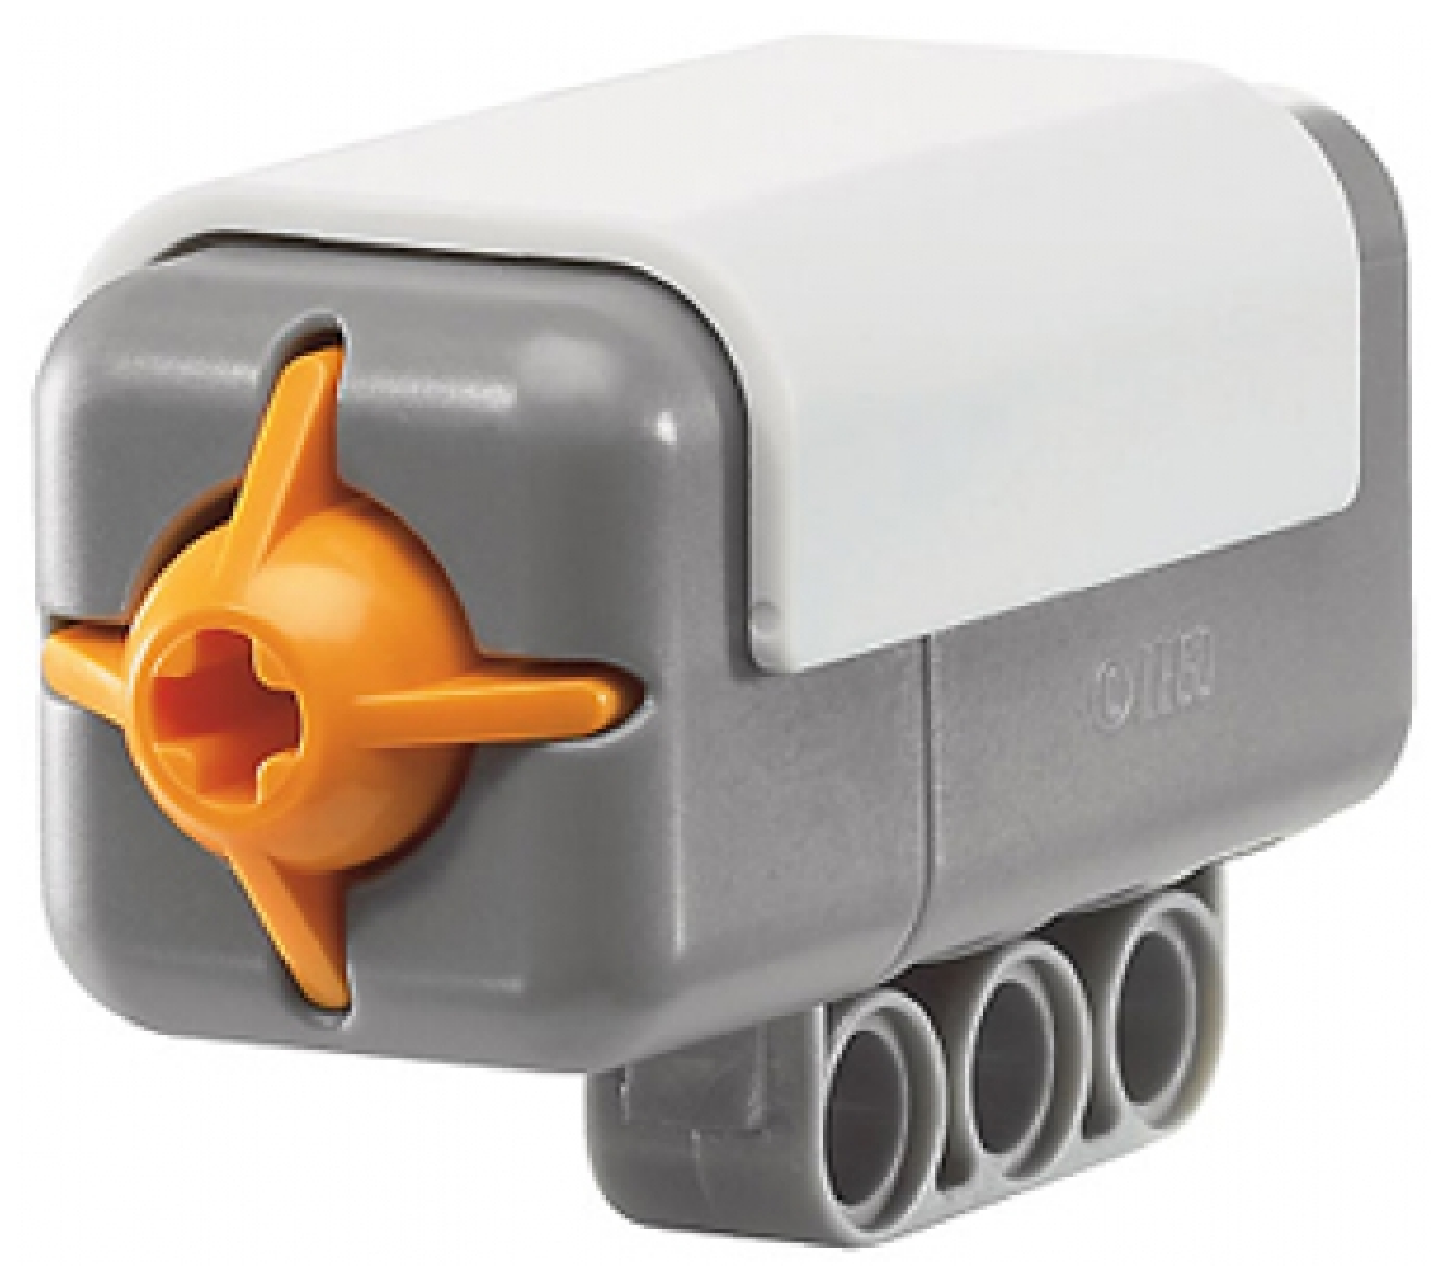
\includegraphics[scale=0.2]{figuras/sensorToque.eps}
					\caption{Sensor de Toque.}
					\label{img:sensorToque}
				\end{figure}

				A classe \textit{TouchSensor}, que implementa a interface deste sensor, contém apenas um simples método:

				\begin{lstlisting}
					boolean isPressed();
				\end{lstlisting}

			\item \textbf{Sensor ultrasônico:}

				Como apresenta a Figura \ref{img:ultrasonic}, o sensor ultrasônico lembra bastante um par de olhos, apesar de possuir muitas características em comum com um sensor de som, em vez de uma câmera, por exemplo. Isso se dá pela estratégia de funcionamento do sensor, o qual emite um sinal sonoro que reflete em obstáculos à frente, retornando ao sensor. A partir da análise do tempo percorrido pelo sinal sonoro, é possível estimar a distância do objeto analisado, em relação ao robô.

				\begin{figure}[H]
					\centering
					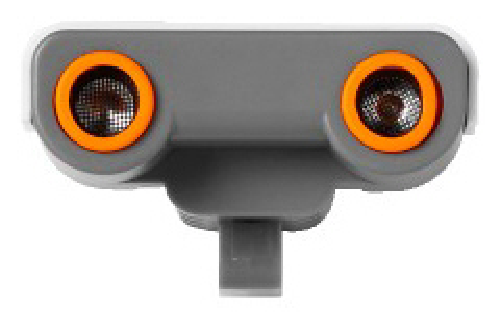
\includegraphics[scale=0.5]{figuras/ultrasonic.eps}
					\caption{Sensor Ultrasônico.}
					\label{img:ultrasonic}
				\end{figure}

				Este sensor é capaz de identificar distâncias de até dois metros e meio, mais especificamente 255 centímetros. Porém, sua utilização em distâncias tão grandes não é recomendada por \cite{legonxj}, devido a grande margem de erro presentes em medições como esta. De acordo com \cite{legonxj}, este sensor possui, em distâncias de aproximadamente 180 centímetros, uma margem de erro de mais ou menos três centímetros (\textit{+/- 3}). Sua margem de erro é proporcional à distância entre robô e obstáculo.

				Outra característica importante do funcionamento deste sensor é a emissão de sinais no formato de cone, como apresenta a Figura \ref{img:cone2}\footnote{http://arcbotics.com/products/sparki/parts/ultrasonic-range-finder/}.


				\begin{figure}[H]
					\centering
					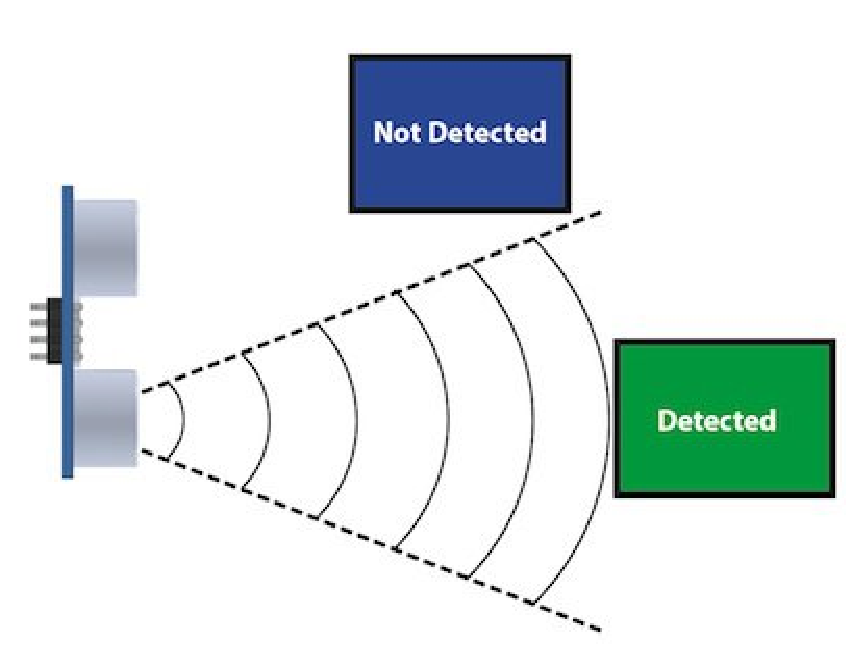
\includegraphics[scale=0.7]{figuras/cone2.eps}
					\caption{Emissão do Sinal Ultrasônico.}
					\label{img:cone2}
				\end{figure}

				O cone formado pela emissão do sinal segue uma angulação de 30º, ou seja, em uma distância de 180 centímetros, o cone possui um diâmetro de 90 centímetros. Desse modo, deve-se levar em consideração a incapacidade de identificar pequenas irregularidades em obstáculos, como fendas e buracos.

				Durante o desenvolvimento da prova de conceito, observou-se com mais precisão a característica descrita acima, levando à alteração da proposta do trabalho, em relação ao ambiente utilizado. Inicialmente, o ambiente proposto se baseava no tapete de missões \textit{Nature's Fury}, utilizado como um dos desafios do torneio \textit{First Lego League}\footnote{http://www.firstlegoleague.org/}. Um exemplo deste ambiente pode ser visualizado na Figura \ref{img:tapete}.

				\begin{figure}[H]
					\centering
					\includegraphics[scale=0.4]{figuras/tapete.eps}
					\caption[Ambiente Proposto Inicialmente]{Ambiente utilizado.}
					\label{img:tapete}
				\end{figure}

				Os problemas referentes aos cantos, buracos e fendas encontrados durante a realização da prova de conceito mostraram o grande impacto desta característica do sonar no mapeamento de ambientes pequenos, como o utilizado. Desse modo, optou-se por modificar o ambiente a ser utilizado durante a segunda etapa deste trabalho. O ambiente será baseado em cômodos reais, como quartos, salas ou escritórios. O critério inicial para utilização do ambiente é referente a área de navegação disponivel, devendo ser de, pelo menos, 2 metros quadrados.

		\end{itemize}

		\subsubsection{Computador Central NXT (Brick)} % (fold)
		\label{sub:brick}

			O robô utilizado durante esta prova de conceito e durante o desenvolvimento da solução proposta, é da família Mindstorm NXT, da Lego. O computador central, de acordo com \cite{legonxj}, possui uma área de 7,2 x 11,2 centímetros, com um processador \textit{Atmel 32-bit ARM} de 48 MHz de frequência, memória RAM de 64 KB e 256 KB de memória \textit{flash}.

			Estas limitações de memória e processamento foram contornadas a partir da utilização da arquitetura de processamento remoto, como foi definido na seção \ref{sec:adaptação_e_implementação}, já como um resultado da revisão sistemática apresentada na seção \ref{sec:revisão_sistemática}.
